\documentclass[10pt]{article}
\usepackage{epstopdf,caption,subcaption,graphicx,xcolor,hyperref}
\usepackage{tikz}
\usepackage{pgfgantt}
\usetikzlibrary{shapes,arrows,fit,calc,positioning}
\usetikzlibrary{decorations.pathreplacing}

\begin{document}

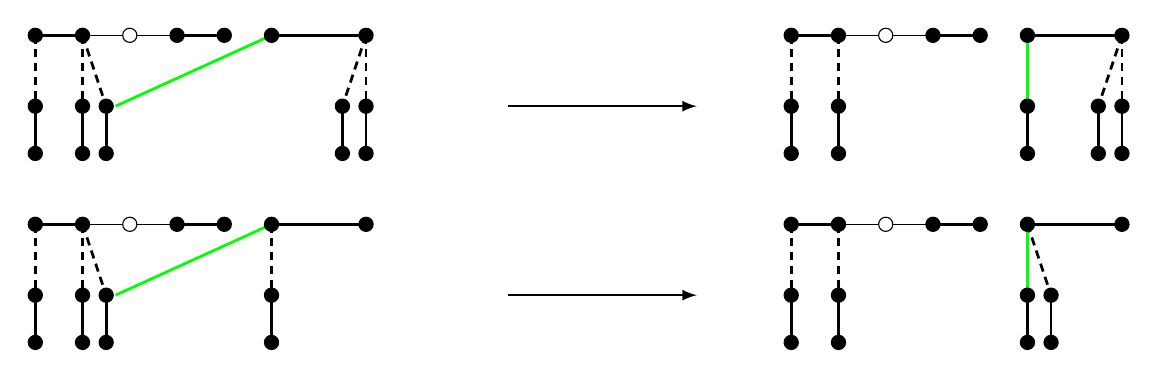
\begin{tikzpicture}[scale=0.6,transform shape]

% the first line

\draw [thick, line width = 1pt] (-8, -6) -- (-7, -6);
\draw [thick, line width = 1pt] (-5, -6) -- (-4, -6);
\draw [thin, line width = 0.5pt] (-7, -6) -- (-6, -6);
\draw [thin, line width = 0.5pt] (-6, -6) -- (-5, -6);
\draw [densely dashed, line width = 1pt] (-8, -6) -- (-8,-7.5);
\draw [thick, line width = 1pt] (-8, -7.5) -- (-8, -8.5);
\draw [densely dashed, line width = 1pt] (-7, -6) -- (-7, -7.5);
\draw [thick, line width = 1pt] (-7, -7.5) -- (-7, -8.5);
\draw [densely dashed, line width = 1pt] (-7, -6) -- (-6.5,-7.5);
\draw [thick, line width = 1pt] (-6.5, -7.5) -- (-6.5, -8.5);
\filldraw (-8, -6) circle(.15);
\filldraw (-7, -6) circle(.15);
\filldraw[fill = white] (-6, -6) circle(.15);
\filldraw (-5, -6) circle(.15);
\filldraw (-4, -6) circle(.15);
\filldraw (-8,-7.5) circle(.15);
\filldraw (-8,-8.5) circle(.15);
\filldraw (-7,-7.5) circle(.15);
\filldraw (-7,-8.5) circle(.15);
\filldraw (-6.5,-7.5) circle(.15);
\filldraw (-6.5,-8.5) circle(.15);

\draw [thick, line width = 1pt, color=green] (-6.3, -7.5) -- (-3, -6);

\draw [thick, line width = 1pt] (-3, -6) -- (-1, -6);
\draw [densely dashed, line width = 1pt] (-1, -6) -- (-1,-7.5);
\draw [thick, line width = 1pt] (-1, -7.5) -- (-1, -8.5);
\draw [densely dashed, line width = 1pt] (-1, -6) -- (-1.5,-7.5);
\draw [thick, line width = 1pt] (-1.5, -7.5) -- (-1.5, -8.5);
\filldraw (-3, -6) circle(.15);
\filldraw (-1, -6) circle(.15);
\filldraw (-1,-7.5) circle(.15);
\filldraw (-1,-8.5) circle(.15);
\filldraw (-1.5,-7.5) circle(.15);
\filldraw (-1.5,-8.5) circle(.15);

\draw [-latex, thick] (2, -7.5) to (6, -7.5);

\draw [thick, line width = 1pt] (8, -6) -- (9, -6);
\draw [thick, line width = 1pt] (11, -6) -- (12,-6);
\draw [thin, line width = 0.5pt] (9, -6) -- (10, -6);
\draw [thin, line width = 0.5pt] (10, -6) -- (11, -6);
\draw [densely dashed, line width = 1pt] (8, -6) -- (8, -7.5);
\draw [thick, line width = 1pt] (8, -7.5) -- (8, -8.5);
\draw [densely dashed, line width = 1pt] (9, -6) -- (9, -7.5);
\draw [thick, line width = 1pt] (9, -7.5) -- (9, -8.5);
\filldraw (8, -6) circle(.15);
\filldraw (9, -6) circle(.15);
\filldraw[fill = white] (10, -6) circle(.15);
\filldraw (11, -6) circle(.15);
\filldraw (12, -6) circle(.15);
\filldraw (8, -7.5) circle(.15);
\filldraw (8, -8.5) circle(.15);
\filldraw (9, -7.5) circle(.15);
\filldraw (9, -8.5) circle(.15);


\draw [thick, line width = 1pt] (13, -6) -- (15, -6);
\draw [thick, line width = 1pt, color=green] (13, -6) -- (13,-7.5);
\draw [thick, line width = 1pt] (13, -7.5) -- (13, -8.5);
\draw [densely dashed, line width = 1pt] (15, -6) -- (15,-7.5);
\draw [thick, line width = 1pt] (15, -7.5) -- (15, -8.5);
\draw [densely dashed, line width = 1pt] (15, -6) -- (14.5,-7.5);
\draw [thick, line width = 1pt] (14.5, -7.5) -- (14.5, -8.5);
\filldraw (13, -6) circle(.15);
\filldraw (15, -6) circle(.15);
\filldraw (13,-7.5) circle(.15);
\filldraw (13,-8.5) circle(.15);
\filldraw (14.5,-7.5) circle(.15);
\filldraw (14.5,-8.5) circle(.15);
\filldraw (15,-7.5) circle(.15);
\filldraw (15,-8.5) circle(.15);

% the second line

\draw [thick, line width = 1pt] (-8, -10) -- (-7, -10);
\draw [thick, line width = 1pt] (-5, -10) -- (-4, -10);
\draw [thin, line width = 0.5pt] (-7, -10) -- (-6, -10);
\draw [thin, line width = 0.5pt] (-6, -10) -- (-5, -10);
\draw [densely dashed, line width = 1pt] (-8, -10) -- (-8,-11.5);
\draw [thick, line width = 1pt] (-8, -11.5) -- (-8, -12.5);
\draw [densely dashed, line width = 1pt] (-7, -10) -- (-7, -11.5);
\draw [thick, line width = 1pt] (-7, -11.5) -- (-7, -12.5);
\draw [densely dashed, line width = 1pt] (-7, -10) -- (-6.5,-11.5);
\draw [thick, line width = 1pt] (-6.5, -11.5) -- (-6.5, -12.5);
\filldraw (-8, -10) circle(.15);
\filldraw (-7, -10) circle(.15);
\filldraw[fill = white] (-6, -10) circle(.15);
\filldraw (-5, -10) circle(.15);
\filldraw (-4, -10) circle(.15);
\filldraw (-8,-11.5) circle(.15);
\filldraw (-8,-12.5) circle(.15);
\filldraw (-7,-11.5) circle(.15);
\filldraw (-7,-12.5) circle(.15);
\filldraw (-6.5,-11.5) circle(.15);
\filldraw (-6.5,-12.5) circle(.15);

\draw [thick, line width = 1pt, color=green] (-6.3, -11.5) -- (-3, -10);

\draw [thick, line width = 1pt] (-3, -10) -- (-1, -10);
\draw [densely dashed, line width = 1pt] (-3, -10) -- (-3,-11.5);
\draw [thick, line width = 1pt] (-3, -11.5) -- (-3, -12.5);
\filldraw (-3, -10) circle(.15);
\filldraw (-1, -10) circle(.15);
\filldraw (-3,-11.5) circle(.15);
\filldraw (-3,-12.5) circle(.15);


\draw [-latex, thick] (2, -11.5) to (6, -11.5);

\draw [thick, line width = 1pt] (8, -10) -- (9, -10);
\draw [thick, line width = 1pt] (11, -10) -- (12,-10);
\draw [thin, line width = 0.5pt] (9, -10) -- (10, -10);
\draw [thin, line width = 0.5pt] (10, -10) -- (11, -10);
\draw [densely dashed, line width = 1pt] (8, -10) -- (8, -11.5);
\draw [thick, line width = 1pt] (8, -11.5) -- (8, -12.5);
\draw [densely dashed, line width = 1pt] (9, -10) -- (9, -11.5);
\draw [thick, line width = 1pt] (9, -11.5) -- (9, -12.5);
\filldraw (8, -10) circle(.15);
\filldraw (9, -10) circle(.15);
\filldraw[fill = white] (10, -10) circle(.15);
\filldraw (11, -10) circle(.15);
\filldraw (12, -10) circle(.15);
\filldraw (8, -11.5) circle(.15);
\filldraw (8, -12.5) circle(.15);
\filldraw (9, -11.5) circle(.15);
\filldraw (9, -12.5) circle(.15);

\draw [thick, line width = 1pt] (13, -10) -- (15, -10);
\draw [thick, line width = 1pt, color=green] (13, -10) -- (13,-11.5);
\draw [thick, line width = 1pt] (13, -11.5) -- (13, -12.5);
\draw [densely dashed, line width = 1pt] (13, -10) -- (13.5,-11.5);
\draw [thick, line width = 1pt] (13.5, -11.5) -- (13.5, -12.5);
\filldraw (13, -10) circle(.15);
\filldraw (15, -10) circle(.15);
\filldraw (13,-11.5) circle(.15);
\filldraw (13,-12.5) circle(.15);
\filldraw (13.5,-11.5) circle(.15);
\filldraw (13.5,-12.5) circle(.15);

\end{tikzpicture}

\end{document}